% v2 (resubmission). Build: pdflatex main.tex && bibtex main && pdflatex main.tex x2
% Every \tbd{} is a number that comes from `python -m eval.analyze` over the
% 5-seed v2 run; none may remain at submission (grep -n tbd sections/*.tex).
\documentclass[11pt]{article}

\usepackage[margin=1in]{geometry}
\usepackage{graphicx}
\usepackage{subcaption}
\usepackage{booktabs}
\usepackage{amsmath,amssymb,amsthm}
\usepackage{hyperref}
\usepackage{xcolor}

\newcommand{\tbd}[1]{\textcolor{red}{#1}}
\newtheorem{proposition}{Proposition}
% Identifying links live here so the anonymous TMLR build (paper_tmlr/) can
% withhold them while sharing these section files.
\newcommand{\demourl}{\url{https://va-uncertainty-demo.vercel.app}}
\newcommand{\codestatement}{Code, configs, predictions, and checkpoints:
\url{https://github.com/Hassan-Naeem-code/Emotion-Modelling}.}

\title{Two Axes, One Guarantee:\\
       Joint Conformal Uncertainty for Valence--Arousal Estimation,\\
       and Where It Breaks}
\author{Hassan Naeem\\
        \normalsize Independent Researcher\\
        \normalsize \texttt{https://hassan-naeem.com}}
\date{\today}

\begin{document}
\maketitle

\begin{abstract}
Uncertainty-aware affect estimators increasingly attach prediction intervals to
their valence and arousal (VA) outputs, typically by calibrating each axis
separately. We show that this common practice gives a guarantee about the wrong
object. A VA estimate is a single point on the circumplex, but per-axis
intervals at a nominal $90\%$ jointly contain the true point only
$86\%$ of the time on AffectNet, and the shortfall is not evenly
spread: the worst-covered expression falls to $78$--$84\%$. We replace the
per-axis score with a single variance-normalised max-score that yields a
rectangular VA region with a finite-sample joint guarantee. It restores nominal
joint coverage and is up to $13\%$ smaller than the Bonferroni correction
that achieves the same guarantee. We then ask where any such guarantee breaks.
AffectNet's \emph{contempt} expression is absent from the training and
calibration data of the release we study, which makes it a natural unseen
expression. On it, every method we evaluate loses its guarantee (joint coverage
$30$--$39\%$), and none of five uncertainty estimators (heteroscedastic
Gaussian, deep evidential regression, MC-dropout, and deep ensembles of each)
flags it reliably (AUROC $\le0.60$); ensembles even lower its coverage.
Feature-space novelty detectors fail as well, because contempt is not an unusual
input: its nearest training faces are mostly happy and neutral, and only its
label is new. Results are over five seeds and hold on a second backbone, with
proper scoring rules, a calibration split that is never used for model selection,
and a corruption shift. Joint coverage is cheap to obtain and should be the
default; detecting unseen expressions remains open.
\end{abstract}

\section{Introduction}

Facial affect is commonly estimated as a point in the two-dimensional
valence--arousal (VA) plane of the circumplex model~\cite{russell1980circumplex},
rather than as one of a few discrete categories. A growing line of work attaches
uncertainty to these estimates, through heteroscedastic likelihoods, deep
evidential regression~\cite{amini2020evidential,wu2023deer}, or ensembles, and
converts that uncertainty into prediction intervals by split conformal
calibration~\cite{vovk2005algorithmic,lei2018distribution}. The appeal is a
finite-sample guarantee: on exchangeable data, a $90\%$ interval contains the
truth at least $90\%$ of the time, whatever the model.

That guarantee is only as useful as the event it is stated about. In practice
the intervals are calibrated per axis, one for valence and one for arousal, and
each comes with its own marginal guarantee. But a downstream consumer of a VA
estimate (an abstention rule, a display, a decision) uses the \emph{pair}. The
event that matters is that the true point lies in the predicted region, and two
marginal $90\%$ guarantees imply only $80\%$ for that event. The question of
which event the guarantee is about, and for whom it holds, is the subject of
this paper.

\paragraph{Contributions.}
\begin{enumerate}
  \item \textbf{A diagnosis.} On AffectNet~\cite{mollahosseini2017affectnet},
        per-axis conformal intervals at nominal $90\%$ jointly cover the true VA
        point only $85$--$86\%$ of the time, across every uncertainty method we test.
        Coverage is also uneven across expressions, with the worst seen expression
        at $78$--$84\%$ depending on the predictor.
  \item \textbf{A simple fix with a guarantee.} A single max-normalised
        nonconformity score gives a rectangular VA region with finite-sample
        joint coverage (Proposition~\ref{prop:joint}). It restores nominal joint
        coverage, improves the worst-expression coverage, and is up to $13\%$ smaller
        than the Bonferroni correction that gives the same guarantee.
  \item \textbf{Where the guarantee breaks.} The AffectNet release we study
        contains \emph{contempt} only in its test split, giving a natural unseen
        expression. There the guarantee fails for every method
        ($30$--$39\%$ coverage), and no uncertainty estimator we evaluate
        flags it reliably. This is a concrete, reproducible instance of the
        limits of distribution-free inference~\cite{barber2021limits} in affect.
  \item \textbf{A clean, broader benchmark.} Five uncertainty methods
        (deterministic, Gaussian, deep evidential regression, MC-dropout, deep
        ensembles) over five seeds, scored with proper scoring
        rules~\cite{gneiting2007strictly} as well as calibration error, with a
        conformal calibration split that is never used for model selection.
\end{enumerate}

\paragraph{Scope.} We study still images and a single dataset family. The claims
are about what calibrated VA uncertainty does and does not guarantee, not about
state-of-the-art accuracy, and we position our predictor against published
results in Section~\ref{sec:results}. The system is intended for estimating a
consenting user's own state; Section~\ref{sec:ethics} discusses its limits.

\section{Related Work}

\paragraph{Dimensional affect estimation.} The circumplex
model~\cite{russell1980circumplex} represents affect by continuous valence and
arousal. AffectNet~\cite{mollahosseini2017affectnet} annotates roughly a million
in-the-wild faces with both categorical expressions and VA, and
AFEW-VA~\cite{kossaifi2017afew,dhall2012afew} and Aff-Wild2~\cite{kollias2019affwild2} provide
VA for video, EmoBank~\cite{buechel2017emobank} for text, and DEAM~\cite{aljanaki2017deam}
for music. Strong image-based VA estimators such as
EmoNet~\cite{toisoul2021estimation} report concordance (CCC) as the main metric;
we do the same, but our object of study is the uncertainty attached to the
estimate.

\paragraph{Uncertainty for emotion.} Label disagreement between annotators makes
affect a natural setting for uncertainty estimation. Wu et
al.~\cite{wu2023deer} apply deep evidential regression to speech emotion
attributes and model annotator disagreement as aleatoric uncertainty. We use the
same family of models for faces but focus on what the resulting intervals
guarantee, and for which inputs.

\paragraph{Predictive uncertainty in deep networks.} MC-dropout~\cite{gal2016dropout}
and deep ensembles~\cite{lakshminarayanan2017simple} estimate epistemic
uncertainty from the disagreement of stochastic or independently trained models;
under dataset shift, ensembles are usually the strongest of the common
methods~\cite{ovadia2019trust}. Out-of-distribution detectors instead score the
input's features, for example by Mahalanobis distance~\cite{lee2018simple} or
nearest-neighbour distance~\cite{sun2022knn}. Deep evidential
regression~\cite{amini2020evidential} obtains aleatoric and epistemic terms in
one forward pass from a Normal--Inverse-Gamma output, though Meinert et
al.~\cite{meinert2023unreasonable} show that its epistemic term is a heuristic
rather than a principled quantity. Our results on an unseen expression are
consistent with that critique. We evaluate with proper scoring
rules~\cite{gneiting2007strictly} (NLL, CRPS) in addition to quantile
calibration error~\cite{kuleshov2018calibrated}, since the latter can be low for
an uninformative predictor.

\paragraph{Conformal prediction.} Split conformal
prediction~\cite{vovk2005algorithmic,lei2018distribution,angelopoulos2021gentle}
gives finite-sample marginal coverage under exchangeability. For multi-output
regression, per-output intervals with a union-bound (Bonferroni) correction are
valid but conservative, and copula-based methods~\cite{messoudi2021copula} model
the dependence between outputs to tighten the joint region; ellipsoidal
regions~\cite{messoudi2022ellipsoidal} use a Mahalanobis score, and
representation-learning approaches~\cite{feldman2023calibrated} learn
non-convex regions. Our max-score region is a simpler member of this family,
with no dependence model to fit, and we compare against the copula and
ellipsoidal constructions directly. Conditional
coverage over groups can be obtained by Mondrian conformal
prediction~\cite{vovk2012conditional} and is a fairness
requirement~\cite{romano2020malice}; with many groups and little data per
group, groups can be clustered by their score
distributions~\cite{ding2023class}, and coverage can be guaranteed over a
whole class of covariate shifts or overlapping
groups~\cite{gibbs2025conditional}. All of these need calibration data from
the group, or at least a group that is defined in advance. Exact conditional coverage for arbitrary
inputs is impossible without assumptions~\cite{barber2021limits}, and coverage
under shift needs reweighting, for covariate shift~\cite{tibshirani2019covariate}
and for label shift~\cite{podkopaev2021label}, whose milder form is present in
our data, where the calibration split is class-balanced and the test split is
not. An expression
absent from the calibration data is the extreme case: there is nothing to
reweight or to calibrate a group on, which is the setting of our unseen-expression
experiment.

\section{Method}
\label{sec:method}

\subsection{Predictors}
A shared ImageNet-pretrained EfficientNet-B0 encoder maps a face crop to a feature
vector, followed by one of three heads predicting VA in $[-1,1]^2$. The
\textbf{deterministic} head is trained with MSE and has no uncertainty. The
\textbf{Gaussian} head predicts a mean $\hat\mu_d$ and variance $\hat\sigma^2_d$
per axis $d\in\{v,a\}$ and is trained with the Gaussian NLL. The
\textbf{evidential} head~\cite{amini2020evidential} predicts
Normal--Inverse-Gamma parameters $(\gamma,\nu,\alpha,\beta)$ per axis, with
predictive mean $\gamma$ and predictive variance
$\beta(1+\nu)/(\nu(\alpha-1))$, the sum of its aleatoric term $\beta/(\alpha-1)$
and epistemic term $\beta/(\nu(\alpha-1))$. Its predictive distribution is a
Student-$t$ with $2\alpha$ degrees of freedom, which we use for its NLL.

From these we form two further methods without additional training.
\textbf{MC-dropout}~\cite{gal2016dropout} keeps the encoder's dropout ($p=0.2$,
the training rate) active for $20$ passes of the evidential model; its variance is
the mean predicted variance plus the variance of the pass means.
\textbf{Deep ensembles}~\cite{lakshminarayanan2017simple} combine the five
independently seeded models of one head, moment-matched in the same way. All
methods thus output a mean $\hat\mu(x)\in\mathbb{R}^2$ and a scale
$\hat\sigma(x)\in\mathbb{R}^2_{>0}$; for the deterministic head we set
$\hat\sigma\equiv 1$, which reduces every construction below to plain
absolute-residual conformal prediction.

\subsection{Per-axis conformal intervals (the common practice)}
Given a calibration set $\{(x_i,y_i)\}_{i=1}^n$ exchangeable with the test data,
the per-axis construction computes normalised scores
$s_{i,d}=|y_{i,d}-\hat\mu_d(x_i)|/\hat\sigma_d(x_i)$, takes
$q_d$ as the $\lceil(n{+}1)(1-\alpha)\rceil$-th smallest $s_{i,d}$, and outputs
$C_d(x)=\hat\mu_d(x)\pm q_d\,\hat\sigma_d(x)$. Each axis is covered with
probability at least $1-\alpha$. The VA point is covered when \emph{both} are,
which the union bound only guarantees with probability $1-2\alpha$.

\subsection{Joint conformal region}
We use one score per sample, the larger of the two normalised residuals,
\begin{equation}
  s_i=\max_{d\in\{v,a\}}\frac{|y_{i,d}-\hat\mu_d(x_i)|}{\hat\sigma_d(x_i)},
  \label{eq:maxscore}
\end{equation}
take $q$ as its $\lceil(n{+}1)(1-\alpha)\rceil$-th smallest value, and output the
rectangle $C(x)=\prod_{d}[\hat\mu_d(x)\pm q\,\hat\sigma_d(x)]$.

\begin{proposition}\label{prop:joint}
If the calibration and test pairs are exchangeable, then
$\Pr\{y\in C(x)\}\ge 1-\alpha$.
\end{proposition}
\begin{proof}
$y\in C(x)$ if and only if $s(x,y)\le q$, where $s$ is the scalar score of
Eq.~\eqref{eq:maxscore}. The standard split-conformal argument for a scalar score
then applies unchanged~\cite{lei2018distribution}.
\end{proof}

The \textbf{Bonferroni} alternative runs the per-axis construction at level
$\alpha/2$. It has the same guarantee but ignores that the two normalised
residuals are dependent, so it is conservative. The max-score adapts to that
dependence without modelling it. Copula
methods~\cite{messoudi2021copula} instead choose a per-axis level $t$ so that
the two calibration ranks fall below $t$ together with probability $1-\alpha$,
assuming independent axes ($t=\sqrt{1-\alpha}$), a Gaussian copula, or the
empirical copula of the calibration ranks; we compare against all three in
Section~\ref{sec:copula}. The empirical copula is the closest relative: with
ranks in place of $\hat\sigma$-normalised residuals it is a max-score region,
but since the ranks are computed on the calibration set itself its guarantee is
approximate rather than exact. We also compare with the ellipsoidal region of
Messoudi et al.~\cite{messoudi2022ellipsoidal}, a Mahalanobis score on the signed
normalised residuals; we estimate its covariance on one half of the calibration
split and its threshold on the other, so its guarantee is exact. An ellipse
does not factor into one interval per axis, so it cannot report a range for
valence and a range for arousal, which the rectangles can. The region inherits the predictor's
heteroscedasticity through $\hat\sigma$, so uncertain inputs get larger regions,
and it is the same object our on-device demonstrator uses as its abstention
signal.\footnote{Live in-browser demo, with the region drawn on the VA plane:
\demourl. No frames leave the device.}

\subsection{Group coverage and unseen expressions}
Marginal coverage can hide groups that are under-covered~\cite{romano2020malice}.
We report joint coverage separately for each AffectNet expression category and
summarise it by the worst seen category. The categorical labels are used only for
this audit; no model sees them. For inputs whose kind is absent from the
calibration data, no conformal method can promise coverage, so the remaining
safeguard is the uncertainty itself. We measure whether it rises on such inputs by
the AUROC of the total predictive standard deviation
$\sum_d\hat\sigma_d$ for separating them from the seen test inputs.

\subsection{Recalibrating for a new expression}
\label{sec:recal-method}
If $k$ labelled examples of the new expression can be collected, coverage on it
can be restored without retraining. \textbf{Group} recalibration (Mondrian
conformal~\cite{vovk2012conditional}) computes a separate max-score threshold
from those $k$ examples; by Proposition~\ref{prop:joint} applied within the
group, it has joint coverage at least $1-\alpha$ on that expression whenever
$k\ge\lceil 1/\alpha\rceil-1$ ($9$ at $\alpha=0.1$). Because an unseen
expression's error is largely a systematic offset (Section~\ref{sec:loeo}), we
also test \textbf{shift} recalibration: half of the $k$ examples estimate the
mean residual $\bar r$ of the expression, which is subtracted from its
predictions, and the other half calibrate the max-score threshold on the
corrected residuals $|y-\hat\mu-\bar r|/\hat\sigma$. The two halves are
disjoint, so this is again an exact split-conformal guarantee. Neither variant
changes the region of any other expression. Both require knowing which
expression a face belongs to at test time; we return to this limitation in
Section~\ref{sec:recal}.

\section{Experimental Setup}
\label{sec:experiments}

\paragraph{Data.} We use a public redistribution of the AffectNet VA
annotations~\cite{mollahosseini2017affectnet} with its own partition:
$58{,}803$ training, $3{,}500$ validation, and $5{,}000$ test images, each with
continuous VA in $[-1,1]^2$ and a categorical expression label. The partition
differs from the official one in two ways that matter here. First, the training
and validation splits are class-balanced (validation has $500$ images of each of
seven expressions), while the test split follows the natural, heavily imbalanced
distribution (from $2{,}354$ \emph{happy} down to $59$ \emph{disgust}). Second,
\emph{contempt} appears only in the test split ($n=70$). We exploit both: the
first is a label shift between calibration and test data, and the second gives
an unseen expression. All seen-data metrics exclude contempt, which is reported
separately.

\paragraph{Protocol.} We hold out a fixed $5\%$ of the training split
($2{,}940$ images, identical for every run) for checkpoint selection. The
validation split is used \emph{only} for conformal calibration and is never seen
during training or selection, so that calibration and test data are
exchangeable up to the label shift above. (Using one split for both purposes, as
is common, weakens the conformal guarantee.) We set $\alpha=0.1$ throughout.

\paragraph{Training.} All heads share the recipe: AdamW (learning rate
$3\times10^{-4}$, weight decay $10^{-4}$), batch size $64$, gradient clipping at
$1.0$, $6$ epochs with $5\%$ linear warm-up and cosine decay, at
$224\times224$. Augmentation is label-preserving: random resized crops (scale
$0.8$--$1$), horizontal flips, rotations up to $10^\circ$, and mild colour jitter.
It contains no blur, noise, or compression, so the corruptions used at test time
remain unseen. The checkpoint with the lowest held-out training loss is kept (NLL
for the probabilistic heads and MSE for the deterministic one, both proper
scores). Each head is trained with five seeds ($1$--$5$). Training one model
takes about $70$ minutes on an Apple M3 Pro.

\paragraph{Distribution shift.} As a covariate shift with fixed labels, we apply
Gaussian blur, Gaussian noise, brightness, contrast, and JPEG compression to the
test images at severity $3$, cycling through the five types by image index in the
spirit of ImageNet-C~\cite{hendrycks2019benchmarking}. The conformal quantile is
calibrated on clean validation data and applied unchanged to corrupted inputs.

\paragraph{Metrics.} \emph{Accuracy:} CCC per axis and RMSE.
\emph{Probabilistic quality:} NLL and CRPS (proper scoring
rules~\cite{gneiting2007strictly}; CRPS uses the Gaussian with the predicted mean
and variance), and quantile calibration error
(ECE)~\cite{kuleshov2018calibrated}. \emph{Selective prediction:} area under the
risk--coverage curve (AURC). \emph{Coverage:} joint coverage of the true VA point
and mean region area, overall and per expression. \emph{Detection:} AUROC of the
uncertainty for clean versus corrupted inputs, and for seen versus contempt.
Single models are reported as mean $\pm$ standard deviation over five seeds;
ensembles combine the five seeds and are reported once.

\paragraph{Reproducibility.} Each model's per-sample predictions are saved once
(\texttt{eval/dump\_preds.py}), and every number in this paper is computed from
them by one script (\texttt{eval/analyze.py}). The per-sample predictions of all
$20$ model files are released with the code (model outputs and image ids only;
the labels are re-attached from the user's copy of the dataset, which we do not
redistribute), so every table and figure can be recomputed without a GPU
(\texttt{make v2-tables}), and
\texttt{make v2-verify} checks the tables in this paper against them. Code,
configs, predictions, and checkpoints:
\url{https://github.com/Hassan-Naeem-code/Emotion-Modelling}.

\section{Results}
\label{sec:results}

% Every number below comes from results/summary/v2/analysis.json, produced by
% eval/analyze.py over the 5-seed v2 run (and results/summary/v2c for the
% ConvNeXt check, via eval/backbone.py); tables/*.tex are generated by them.

\subsection{Predictors are comparable on accuracy}
Table~\ref{tab:main} reports accuracy and probabilistic quality on the seen test
expressions. The deterministic, evidential, and MC-dropout predictors are within
seed noise of each other (CCC $0.712$--$0.720$, std $\approx0.01$); the Gaussian
head is consistently weaker ($0.693$), and ensembling five seeds adds about
$0.01$ for either head. Our evidential model reaches CCC $0.829$ on valence and
$0.610$ on arousal. For context, the AffectNet authors' baseline reports
$0.541$ and $0.450$ on their test set~\cite{mollahosseini2017affectnet}, and
EmoNet~\cite{toisoul2021estimation} reports $0.82$ and $0.75$ on a cleaned test
set. These comparisons are indicative only, since the partitions differ (see
Section~\ref{sec:experiments}). The point is that the coverage results below rest
on a predictor of representative strength. On proper scores, the evidential head
has the best NLL ($-0.067$) and the evidential ensemble the best CRPS
($0.135$). Calibration error disagrees: the ensembles have the \emph{worst} ECE
($0.043$--$0.044$, against $0.022$--$0.027$ for single models) despite better
proper scores, a reminder that ECE alone does not rank predictors.

\begin{table}[h]
  \centering\small
  \resizebox{\linewidth}{!}{\begin{tabular}{lccccccc}
\toprule
Method & CCC-V$\uparrow$ & CCC-A$\uparrow$ & RMSE$\downarrow$ & NLL$\downarrow$ & CRPS$\downarrow$ & ECE$\downarrow$ & AURC$\downarrow$ \\
\midrule
Deterministic & 0.822$_{\pm.008}$ & 0.602$_{\pm.011}$ & 0.269$_{\pm.003}$ & -- & -- & -- & -- \\
Gaussian & 0.807$_{\pm.009}$ & 0.579$_{\pm.022}$ & 0.274$_{\pm.003}$ & 0.006$_{\pm.013}$ & 0.144$_{\pm.002}$ & \textbf{0.022}$_{\pm.011}$ & 0.041$_{\pm.001}$ \\
Evidential & 0.829$_{\pm.006}$ & 0.610$_{\pm.010}$ & 0.270$_{\pm.003}$ & \textbf{-0.067}$_{\pm.015}$ & 0.138$_{\pm.002}$ & 0.026$_{\pm.010}$ & 0.039$_{\pm.002}$ \\
MC-dropout & 0.829$_{\pm.006}$ & 0.610$_{\pm.011}$ & 0.270$_{\pm.003}$ & 0.002$_{\pm.017}$ & 0.138$_{\pm.002}$ & 0.027$_{\pm.010}$ & 0.039$_{\pm.002}$ \\
Gaussian ens. & 0.817 & 0.595 & 0.266 & -0.031 & 0.139 & 0.044 & 0.038 \\
Evidential ens. & \textbf{0.838} & \textbf{0.624} & \textbf{0.262} & -0.053 & \textbf{0.135} & 0.043 & \textbf{0.036} \\
\bottomrule
\end{tabular}
}
  \caption{Accuracy and probabilistic quality on seen test expressions.
  Mean$_{\pm\text{std}}$ over five seeds; ensembles combine the five seeds.
  NLL and CRPS are proper scores (lower is better).}
  \label{tab:main}
\end{table}

\subsection{Per-axis intervals under-cover the VA point}
Table~\ref{tab:coverage} compares the three conformal constructions on top of
every predictor. With per-axis intervals, joint coverage is $0.853$--$0.861$,
four to five points below nominal, for every predictor and with seed std below
$0.01$: the shortfall is systematic, not noise. The max-score region restores it
($0.917$--$0.930$), as does Bonferroni ($0.922$--$0.941$), but the max-score
region is smaller in every case: by $11\%$ for the evidential model ($1.39$
versus $1.57$), $13\%$ for the evidential ensemble, $7\%$ for the Gaussian head,
and $3\%$ for the deterministic one. The saving grows with the quality of
$\hat\sigma$, as expected, since a constant scale leaves no dependence between
the normalised residuals for the max-score to exploit beyond that of the raw
residuals.

The gap is also uneven across expressions (Figure~\ref{fig:per_emotion}). Under
per-axis intervals, six of the seven seen expressions are below nominal for the
evidential model, and \emph{sad} is covered least ($0.836$); for the
deterministic model it falls to $0.784$. The max-score region raises the
worst seen expression to $0.905$ for the evidential model, but only to $0.868$
for the deterministic one: with a constant scale, the region has the same shape
for every face, so it cannot widen where errors are larger. Learned
uncertainty is what makes group coverage close to uniform. Coverage above
nominal on the overall test set reflects the label shift between the
class-balanced calibration split and the imbalanced test split, which
over-represents \emph{happy}, an expression with narrow residuals.

\begin{table}[h]
  \centering\small
  \resizebox{\linewidth}{!}{\begin{tabular}{lcccccccc}
\toprule
 & \multicolumn{2}{c}{Per-axis} & \multicolumn{2}{c}{Bonferroni} & \multicolumn{2}{c}{Max-score (ours)} & \multicolumn{2}{c}{Worst / Shift (ours)} \\
Method & Joint & Area & Joint & Area & Joint & Area & Worst & Shift \\
\midrule
Deterministic & 0.860$_{\pm.005}$ & 0.991$_{\pm.015}$ & 0.922$_{\pm.005}$ & 1.561$_{\pm.028}$ & 0.920$_{\pm.005}$ & 1.517$_{\pm.023}$ & 0.868$_{\pm.014}$ & 0.809$_{\pm.047}$ \\
Gaussian & 0.853$_{\pm.007}$ & 0.792$_{\pm.021}$ & 0.929$_{\pm.007}$ & 1.281$_{\pm.048}$ & 0.921$_{\pm.005}$ & 1.186$_{\pm.039}$ & 0.879$_{\pm.019}$ & 0.879$_{\pm.066}$ \\
Evidential & 0.861$_{\pm.003}$ & 0.826$_{\pm.018}$ & 0.941$_{\pm.003}$ & 1.567$_{\pm.057}$ & 0.930$_{\pm.005}$ & 1.388$_{\pm.048}$ & \textbf{0.905}$_{\pm.007}$ & 0.920$_{\pm.023}$ \\
MC-dropout & 0.860$_{\pm.004}$ & 0.822$_{\pm.016}$ & 0.941$_{\pm.003}$ & 1.566$_{\pm.052}$ & 0.929$_{\pm.004}$ & 1.376$_{\pm.049}$ & 0.904$_{\pm.007}$ & 0.920$_{\pm.023}$ \\
Gaussian ens. & 0.855 & 0.717 & 0.928 & 1.124 & 0.917 & \textbf{1.024} & 0.883 & 0.924 \\
Evidential ens. & 0.860 & 0.721 & 0.937 & 1.348 & 0.924 & 1.178 & \textbf{0.905} & 0.934 \\
\bottomrule
\end{tabular}
}
  \caption{Conformal regions at nominal $90\%$, calibrated on validation. Joint:
  fraction of seen test faces whose true VA point lies in the region. Area: mean
  region area in VA units. Worst: lowest joint coverage across the seven seen
  expressions. Shift: joint coverage on corrupted test images, with the quantile
  calibrated on clean data.}
  \label{tab:coverage}
\end{table}

\begin{figure}[t]
  \centering
  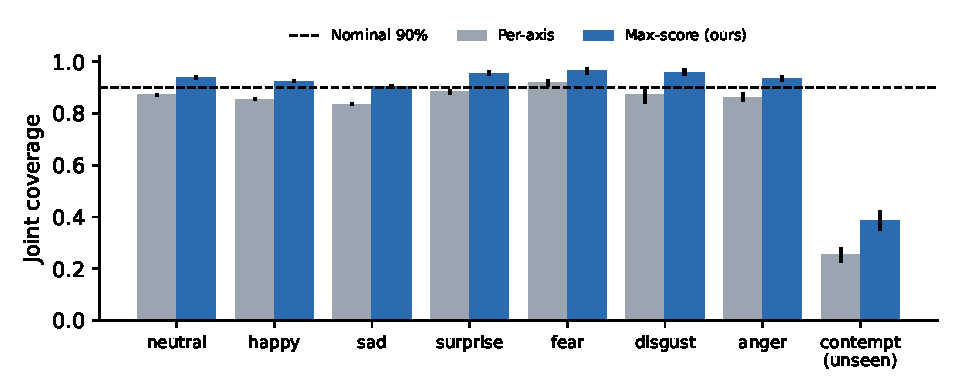
\includegraphics[width=\linewidth]{tables/per_emotion.pdf}
  \caption{Joint coverage of the true VA point per expression (evidential head,
  nominal $90\%$, dashed). Per-axis intervals under-cover most seen expressions;
  the max-score region lifts every seen expression to near or above nominal.
  Contempt, absent from training and calibration, is far below nominal under
  both.}
  \label{fig:per_emotion}
\end{figure}

\subsection{Unseen expressions break every guarantee}
On \emph{contempt}, which no model saw during training or calibration, errors are
$2.5\times$ larger (RMSE $0.65$--$0.68$ versus $0.27$): models place contempt
near neutral, slightly positive valence (mean prediction $(+0.16,+0.10)$ over
seeds), whereas its labels are clearly negative and aroused ($(-0.50,+0.59)$).
Joint coverage collapses to $30$--$39\%$ (Table~\ref{tab:unseen}; per-axis
intervals give $22$--$27\%$). With $n=70$, the $95\%$ Wilson interval is about
$\pm0.11$, so every method is far below nominal. The guarantee is not violated,
since exchangeability does not hold, but a user relying on it would not know
that. The remaining safeguard is the uncertainty itself, and it barely rises: the
AUROC for flagging contempt is $0.58$--$0.60$ for every method. The evidential
epistemic term alone does no better ($0.584$) than total variance ($0.583$),
consistent with the critique of Meinert et al.~\cite{meinert2023unreasonable}.
Ensembles, the usual remedy under shift~\cite{ovadia2019trust}, do not help
either: they leave AUROC unchanged and \emph{lower} contempt coverage ($0.343$
and $0.300$ against $0.386$ and $0.369$ for their members), because their
tighter regions are wrong in the same direction.

\begin{table}[h]
  \centering\small
  \begin{tabular}{lccc}
\toprule
Method & RMSE$\downarrow$ & Joint cov. & AUROC$\uparrow$ \\
\midrule
Deterministic & 0.659$_{\pm.020}$ & 0.386$_{\pm.024}$ & -- \\
Gaussian & 0.654$_{\pm.014}$ & 0.369$_{\pm.046}$ & 0.594$_{\pm.037}$ \\
Evidential & 0.681$_{\pm.013}$ & 0.386$_{\pm.039}$ & 0.583$_{\pm.011}$ \\
MC-dropout & 0.681$_{\pm.013}$ & 0.383$_{\pm.037}$ & 0.583$_{\pm.011}$ \\
Gaussian ens. & \textbf{0.650} & 0.300 & \textbf{0.602} \\
Evidential ens. & 0.678 & 0.343 & 0.583 \\
\bottomrule
\end{tabular}
% Wilson 95% half-width at p=0.4, n=70: 0.112

  \caption{Unseen expression (contempt, $n=70$). RMSE, joint coverage of the
  max-score region, and AUROC of total predictive standard deviation for
  separating contempt from seen test faces (0.5 = chance).}
  \label{tab:unseen}
\end{table}

\subsection{Contempt looks familiar, so input-based detectors fail too}
\label{sec:novelty}
If the predictive uncertainty does not notice contempt, a detector that looks
at the input might. We test three standard feature-space detectors on each
model's penultimate features, fit on $12{,}000$ training images of the seven
seen expressions: Mahalanobis distance to a single Gaussian, the minimum
class-conditional Mahalanobis distance with shared covariance~\cite{lee2018simple},
and the distance to the $50$th nearest training feature after $\ell_2$
normalisation~\cite{sun2022knn}. Each detector's threshold is set on the
validation split so that about $5\%$ of seen faces are flagged, as a deployment
would. Table~\ref{tab:novelty} reports the evidential model; the Gaussian and
deterministic models behave the same.

None of them works. Both Mahalanobis detectors score contempt as \emph{more}
typical than the seen test faces (AUROC $0.44$--$0.47$ across the three heads,
below chance), $k$-NN does no better than the predictive uncertainty
($0.57$--$0.59$), and at the deployment threshold every detector flags at most
$8\%$ of contempt faces. The same detectors do respond to the corrupted images
(AUROC $0.63$--$0.68$, above the predictive uncertainty's $0.58$--$0.60$), so they
are not broken; contempt is simply not unusual as an input. Its nearest training
neighbours are $41\%$ \emph{happy} and $28\%$ \emph{neutral} faces ($\pm3\%$
over all $15$ models), and its distance to the training set matches that of
seen faces. What is novel about contempt is its \emph{label}: a familiar
asymmetric half-smile that annotators rate as clearly negative. A model that
maps it to the valence of its look-alikes is wrong with no signal in its input
or its features, so abstaining on flagged inputs leaves contempt coverage where
it was ($0.39$, ``contempt safe'' in Table~\ref{tab:novelty}). The only remedy we
see is calibration data that contains the expression.

\begin{table}[h]
  \centering\small
  \resizebox{\linewidth}{!}{\begin{tabular}{lccccc}
\toprule
Detector & AUROC$\uparrow$ & Flagged contempt & Flagged seen & Contempt safe & Shift AUROC \\
\midrule
Predictive $\sum_d\hat\sigma_d$ & 0.583$_{\pm.011}$ & 0.054$_{\pm.017}$ & 0.038$_{\pm.003}$ & 0.386$_{\pm.039}$ & 0.604$_{\pm.016}$ \\
Mahalanobis & 0.464$_{\pm.016}$ & 0.011$_{\pm.006}$ & 0.045$_{\pm.005}$ & 0.394$_{\pm.046}$ & 0.662$_{\pm.015}$ \\
Class-cond.\ Mahalanobis & 0.466$_{\pm.016}$ & 0.011$_{\pm.006}$ & 0.045$_{\pm.004}$ & 0.394$_{\pm.046}$ & 0.663$_{\pm.016}$ \\
$k$-NN ($k{=}50$) & 0.571$_{\pm.009}$ & 0.051$_{\pm.007}$ & 0.047$_{\pm.002}$ & 0.391$_{\pm.043}$ & 0.634$_{\pm.007}$ \\
\bottomrule
\end{tabular}
}
  \caption{Detecting the unseen expression (evidential model, five seeds). AUROC
  separates contempt from seen test faces. Flagged: fraction above a threshold
  set on validation to flag about $5\%$ of seen faces. Contempt safe: fraction of
  contempt that is either flagged or covered by the joint region. Shift AUROC:
  clean versus corrupted test images.}
  \label{tab:novelty}
\end{table}

\subsection{Corruption shift}
Under corruption at severity $3$, the evidential model's CCC drops from $0.720$
to $0.595$. The max-score region keeps joint coverage at $0.920$ without
recalibration, while per-axis intervals fall to $0.840$. The deterministic model
degrades far more: its CCC falls to $0.500$ with large variation across seeds
($\pm0.108$), and its region covers only $0.809$, because a constant-width region
cannot widen on degraded inputs. Detecting corrupted inputs from uncertainty is
weak for every method (AUROC $0.58$--$0.62$), yet the evidential scale rises
enough on the inputs where it errs to keep coverage. Corruptions of moderate
severity leave most faces readable, so flat uncertainty on most of them is not
by itself a failure.

\subsection{The findings hold on a second backbone}
\label{sec:backbone}
Table~\ref{tab:backbone} repeats the coverage analysis with ConvNeXt-Tiny. It is
slightly more accurate (CCC $0.713$--$0.732$ against $0.693$--$0.720$), and the
coverage findings carry over. Per-axis intervals again under-cover the VA point
($0.836$--$0.864$) and the max-score region restores it ($0.915$--$0.928$). The
region is smaller than Bonferroni by $13\%$ for the evidential head, $8\%$ for the
Gaussian head and $4\%$ for the deterministic one, the same ordering as with
EfficientNet. Learned uncertainty again lifts the worst seen expression, from
$0.869$ (deterministic) to $0.891$ (evidential). Contempt coverage stays at
$32$--$36\%$ ($30$--$34\%$ for the ensembles), and the AUROC for flagging it stays
at $0.58$--$0.59$: the larger encoder, with ImageNet-22k pretraining, does not
notice the unseen expression either.

One finding does \emph{not} carry over. ConvNeXt is barely affected by the
corruptions (CCC drops by $0.02$, against $0.12$ to $0.21$ for EfficientNet), so
every head, including the deterministic one, keeps joint coverage above $0.90$
under shift. The advantage of learned uncertainty under corruption in
Section~\ref{sec:results} therefore reflects a backbone that degrades, not a
property of the region: it matters when the input shift actually hurts the
predictor.

\begin{table}[h]
  \centering\small
  \resizebox{\linewidth}{!}{\begin{tabular}{llcccccccc}
\toprule
Backbone & Head & CCC & Per-axis & Joint & Area & Area (Bonf.) & Worst & Contempt & Shift \\
\midrule
EfficientNet-B0 ($n=5$) & Deterministic & 0.712$_{\pm.009}$ & 0.860$_{\pm.005}$ & 0.920$_{\pm.005}$ & 1.517$_{\pm.023}$ & 1.561$_{\pm.028}$ & 0.868$_{\pm.014}$ & 0.386$_{\pm.024}$ & 0.809$_{\pm.047}$ \\
 & Gaussian & 0.693$_{\pm.013}$ & 0.853$_{\pm.007}$ & 0.921$_{\pm.005}$ & 1.186$_{\pm.039}$ & 1.281$_{\pm.048}$ & 0.879$_{\pm.019}$ & 0.369$_{\pm.046}$ & 0.879$_{\pm.066}$ \\
 & Evidential & 0.720$_{\pm.008}$ & 0.861$_{\pm.003}$ & 0.930$_{\pm.005}$ & 1.388$_{\pm.048}$ & 1.567$_{\pm.057}$ & 0.905$_{\pm.007}$ & 0.386$_{\pm.039}$ & 0.920$_{\pm.023}$ \\
\midrule
ConvNeXt-Tiny ($n=3$) & Deterministic & 0.732$_{\pm.004}$ & 0.864$_{\pm.006}$ & 0.928$_{\pm.002}$ & 1.461$_{\pm.013}$ & 1.520$_{\pm.013}$ & 0.869$_{\pm.019}$ & 0.324$_{\pm.018}$ & 0.921$_{\pm.003}$ \\
 & Gaussian & 0.713$_{\pm.002}$ & 0.836$_{\pm.006}$ & 0.915$_{\pm.001}$ & 1.034$_{\pm.029}$ & 1.118$_{\pm.044}$ & 0.886$_{\pm.007}$ & 0.329$_{\pm.023}$ & 0.908$_{\pm.001}$ \\
 & Evidential & 0.730$_{\pm.005}$ & 0.857$_{\pm.004}$ & 0.925$_{\pm.005}$ & 1.197$_{\pm.057}$ & 1.371$_{\pm.086}$ & 0.891$_{\pm.009}$ & 0.357$_{\pm.012}$ & 0.919$_{\pm.003}$ \\
\bottomrule
\end{tabular}
}
  \caption{Main claims on two backbones (mean$_{\pm\text{std}}$ over seeds;
  nominal $90\%$). Per-axis: joint coverage of per-axis intervals. Joint and
  Area: max-score region. Area (Bonf.): Bonferroni region with the same
  guarantee. Worst: lowest joint coverage over seen expressions. Contempt and
  Shift: joint coverage of the max-score region on the unseen expression and on
  corrupted images.}
  \label{tab:backbone}
\end{table}

\subsection{Summary}
Across five predictors, five seeds and two backbones, three findings are stable. First,
per-axis intervals miss the VA point about $14\%$ of the time at nominal $10\%$,
for every predictor; the max-score region fixes this at no cost and with regions
up to $13\%$ smaller than Bonferroni. Second, learned uncertainty is what makes
the guarantee useful beyond its marginal form: it lifts the worst seen
expression from $0.868$ to $0.905$ and, when the backbone degrades under
corruption, holds coverage there ($0.920$ versus $0.809$) at equal accuracy. Third, none of this extends to an
expression absent from the calibration data: coverage there is $30$--$39\%$, and
nothing flags it, neither the predictive uncertainty, nor ensembles, nor
feature-space detectors (AUROC $\le0.60$), because the expression looks like
faces the model has seen.

\section{Ethical Considerations}
\label{sec:ethics}

Facial affect inference is a dual-use technology. Much of its deployed use
involves inferring the internal states of people who have not asked for it, which
is what our design is meant to resist. We state our position explicitly.

\paragraph{What the system claims.} It estimates a \emph{perceived} affective
display along valence and arousal, as annotated by human raters. It does not
recover a person's felt emotion, intent, or truthfulness, and the dimensional
target is not a diagnosis. The scientific premise that discrete internal
emotional states can be read off a face is contested~\cite{russell1980circumplex};
we therefore predict the continuous, annotator-defined quantity our labels
actually contain, and attach an interval to every prediction rather than a
confident point.

\paragraph{Intended and excluded uses.} The demonstrator estimates the user's own
state, on their own device, at their request. We explicitly exclude monitoring of
people who are not the operator (employee, student, candidate, or suspect
assessment) and any deception-detection or mental-health screening
application. Abstention is a first-class outcome for exactly this reason: a
system that must always answer invites use in settings where it should not be
used at all.

\paragraph{Privacy.} No imagery or biometric signal leaves the device in the
demonstrator; inference runs in the browser and no frames are transmitted or
stored. We do not redistribute AffectNet, which is registration-gated, and we
commit no image data to the public repository, only metrics and rendered
figures.

\paragraph{Bias and unequal performance.} We report aggregate accuracy and
calibration only. AffectNet's demographic composition is not balanced, and
expression annotation is known to carry cultural and racial bias; aggregate
calibration can therefore hide substantially worse calibration for
under-represented groups. We make no fairness claim, and we regard per-group
calibration as the most important extension of this work: an abstention threshold
calibrated on a population that does not represent the user is a threshold that
fails silently for that user, which is the exact failure mode this paper argues
against.

\section{Conclusion}

A VA estimate is one point in the plane, so its uncertainty should be one region
in the plane. Calibrating valence and arousal separately, as is common, leaves
the guarantee on the wrong event and under-covers the VA point by about
four to five points at nominal $90\%$. One max-normalised score fixes this with a
finite-sample joint guarantee and smaller regions than the Bonferroni correction.
It costs a single line of code, and we recommend it as the default.

The harder finding is where guarantees end. An expression absent from the
calibration data loses coverage under every method we tried, and none of the
uncertainty estimators reliably notices. Conformal methods cannot fix this by
construction, so a deployed affect estimator needs either calibration data that
spans the expressions it will meet or an uncertainty signal that actually rises
on novel ones. We found neither in the standard toolkit, and the reason is
instructive: contempt is not an unusual input but a familiar-looking face with an
unfamiliar meaning, so no signal computed from the input alone can be expected
to flag it.

\paragraph{Limitations.} We study still images from one dataset family and two
backbones (the second with three seeds). A
cross-dataset shift (AFEW-VA, Aff-Wild2) and annotator-level labels would test
whether the uncertainty tracks human disagreement. Our unseen expression has only
$70$ examples, so its coverage estimates carry wide intervals (we report them).
The categorical labels used for the per-expression audit are themselves noisy
annotations of a continuous state.


\bibliographystyle{plain}
\bibliography{refs}

\end{document}
